\documentclass[a4paper, 12pt]{article}

\usepackage[utf8]{inputenc}
\usepackage[T1]{fontenc}
\usepackage{lmodern}
\usepackage[german]{babel}
\usepackage{helvet}
\renewcommand{\familydefault}{\sfdefault}
\usepackage[singlespacing]{setspace}
\usepackage[margin=1in]{geometry}
\usepackage{parskip}
\usepackage{bibgerm}
\usepackage{graphicx}
\usepackage{tcolorbox}
\usepackage{dingbat}
\usepackage{pdfpages}
\usepackage{hyperref}

\newcommand{\leadingzero}[1]{\ifnum #1<10 0\the#1\else\the#1\fi}
\newcommand{\datumVonHeute}{\leadingzero{\day}.\leadingzero{\month}.\the\year}

\newcommand{\haThema}{”latent-space interpolation”}
\newcommand{\haAutor}{Liza Kaladjian}
\newcommand{\haDeckblattTextEins}{Projekt in Fach Advances in Intelligent Systems (ISS)}
\newcommand{\haGutachter}{Dr. Dennis Müller}
\newcommand{\haGutachterText}{Professor für Künstliche Intelligenz und Data Science}

\title{\haThema}
\author{\haAutor}
\date{\today}

\begin{document}

\begin{titlepage}
Hochschule Düsseldorf \\
University of Applied Sciences	
\begin{center}
\vspace{1.5cm}
{\scshape\large \haDeckblattTextEins \par}
\vspace{1cm}
{\scshape\large zum Thema\par}
\vspace{1.5cm}
{\LARGE\bfseries \haThema \par}
\vfill
{Erstellt von:\\ {\bfseries \haAutor} \par}
\vspace{1cm}
\vspace{1cm}
Gutachter:\\ {\bfseries \haGutachter}\\ \haGutachterText
\vfill
\end{center}
\end{titlepage}
\thispagestyle{empty}
\newpage

\tableofcontents
\thispagestyle{empty}
\newpage

\setcounter{page}{1}

\section{Einleitung}
\subsection{Ziel und Motivation}
Meine Faszination für Generative Adversarial Networks (GANs) begann mit meiner alltäglichen Interaktion mit sozialen Medien und dem Internet. Oft begegnete ich beeindruckenden Anwendungen von GANs, ohne zu Beginn zu verstehen, welche Technologie dahintersteckt. Ein prägnantes Beispiel, das mein Interesse entfachte, war eine Herausforderung auf einer Webseite, bei der man auf die Person klicken musste, die real ist. Diese Aufgabe offenbarte mir die erstaunliche Fähigkeit von GANs, Bilder zu erzeugen, die so lebensecht sind, dass sie kaum von echten Fotos zu unterscheiden sind – eine faszinierende Demonstration der Leistungsfähigkeit dieser Technologie.

Diese und andere Anwendungen, wie Deepfakes, zeigen eindrucksvoll, wie GANs in der Lage sind, realistische Bilder und Videos zu generieren, die sich kaum von echten Aufnahmen unterscheiden lassen. Eines der beeindruckendsten Beispiele, das meine Neugier weiter entfachte, war ein \cite{gif_example}, das einen fließenden Übergang zwischen verschiedenen Gesichtern zeigte. Die Fähigkeit von GANs, nahtlose Übergänge und Transformationen zu schaffen, hat mich dazu inspiriert, mehr über diese Technologie zu erfahren und schließlich selbst ein Projekt in diesem Bereich zu starten.

In der heutigen Zeit finden GANs in verschiedenen Bereichen Anwendung, von der Kunst über die Unterhaltungsbranche bis hin zur Wissenschaft. Beispiele hierfür sind:
\begin{itemize}
  \item \textbf{Künstlerische Kreationen}: Künstler nutzen GANs, um einzigartige Kunstwerke zu schaffen, die oft neue Perspektiven und Stile hervorbringen, welche ohne diese Technologie nicht möglich wären.\cite{kunstloft_article}
  \item \textbf{Medizinische Bildgebung}: In der Medizin werden GANs eingesetzt, um realistische medizinische Bilder für Trainingszwecke zu generieren, ohne dabei auf sensible Patientendaten zugreifen zu müssen. \cite{avinci_ai_gans}
\end{itemize}


Diese breiten Anwendungsmöglichkeiten demonstrieren die Vielseitigkeit und das transformative Potenzial von GANs. Mein Ziel in diesem Projekt ist es, ein tieferes Verständnis dieser Technologie zu entwickeln und sie praktisch anzuwenden, um ein eigenes GIF erstellen zu können, das ähnlich ist wie das GIF Beispiel, das mein Interesse ursprünglich geweckt hat.

\subsection{State of the Art bei GANs}
GANs haben sich als weit verbreiteter Ansatz zur Bildsynthese etabliert und dieser Bereich hat durch die Arbeit führender Organisationen wie NVIDIA und verschiedenen Forschungsinitiativen, wie z.B. Midjourney, signifikante Fortschritte erzielt. NVIDIA hat mit seinen StyleGAN-Modellen, insbesondere StyleGAN2 und StyleGAN3, neue Maßstäbe in der Erzeugung hochrealistischer Bilder gesetzt\cite{StyleGAN3, StyleGAN3_Github, StyleGAN2}. Diese Modelle haben bahnbrechende Verbesserungen in der Bildqualität und -konsistenz gezeigt und sind insbesondere für ihre Fähigkeit bekannt, überzeugende und konsistente Gesichtsbilder zu generieren\cite{StyleGAN3, StyleGAN3_Github}.

Das neueste Modell StyleGAN3 ist eine Weiterentwicklung von StyleGAN2 und bringt einige wichtige Verbesserungen mit sich. StyleGAN3 kann zum Beispiel besser mit Kamerabewegungen umgehen, was es besonders nützlich für Video- und Animationsprojekte macht\cite{StyleGAN3_next}.

Die Weiterentwicklungen in der 3D-GAN-Technologie und die Einführung von Transformer-basierten Ansätzen wie TransGAN zeigen das dynamische und sich schnell entwickelnde Feld der GAN-Forschung\cite{jiang2021transgan}. Diese Entwicklungen, zusammen mit den Beiträgen von Midjourney und anderen Forschungsgruppen, zeigen das enorme Potenzial von GANs und dienen als wichtige Inspiration und Benchmark für mein eigenes Projekt.


Obwohl ich in diesem Projekt mein eigenes GAN-Netzwerk von Grund auf entwickeln wollte, war es dennoch faszinierend, den aktuellen Stand der Technik bei GANs zu betrachten. Ich war mir bewusst, dass meine einfacheren Modelle möglicherweise nicht die hochgradige Bildqualität wie die fortgeschrittensten Systeme erreichen würden. Jedoch lag der Fokus meines Projekts darauf, ein grundlegendes Verständnis für die Funktionsweise von GANs zu erlangen. Durch das eigenständige Aufbauen und Trainieren meines Modells konnte ich wertvolle Erfahrungen sammeln und ein tiefes Verständnis für die komplexen Mechanismen und Herausforderungen von GANs entwickeln. Diese Erfahrungen waren für mich enorm wertvoll und ermöglichten es mir, in relativ kurzer Zeit ein funktionsfähiges Modell zu trainieren. Dieser Prozess zeigte mir auch, wie viel Raum für Innovation und Verbesserung in diesem Bereich noch besteht, und motivierte mich, meine Forschung und Entwicklung in diesem faszinierenden Feld der Künstlichen Intelligenz weiter voranzutreiben.

\subsection{Überblick über das Projekt}
Wie bereits erwähnt geht es in diesem Projekt  um GANS , das sich auf die Generierung und Interpolation von Gesichtern konzentriert. Ich habe den CelebA-Datensatz von Kaggle verwendet, der eine breite Palette von Gesichtern enthält. Dieser Datensatz ist ideal für die Training des GANs, da er eine Vielfalt an Gesichtszügen und Ausdrücken bietet und kostenlos verfügbar ist.\footnote{\url{https://www.kaggle.com/datasets/jessicali9530/celeba-dataset}}

Das Projekt besteht aus zwei Hauptkomponenten:
\begin{enumerate}
  \item \textbf{Der Generator (Generator.py)}: Diese Komponente generiert neue, realistische Gesichtsbilder, basierend auf dem CelebA-Datensatz. Es ist faszinierend, wie der Generator aus reinen Daten lebendige Bilder erschafft.
  \item \textbf{Der Kritiker (Critic.py)}: Dieser Teil bewertet die vom Generator erstellten Bilder und hilft dabei, dessen Fähigkeiten zu verbessern, indem er beurteilt, wie realistisch die Bilder sind.
\end{enumerate}

Ein interessanter Aspekt des Projekts ist die \textbf{(Interpolation.py)}, wo ich mit fließenden Übergängen zwischen verschiedenen Gesichtern experimentiere. Der Trainingsprozess, implementiert in \textbf{(Trainloop.py)}, nutzt den CelebA-Datensatz, um sowohl den Generator als auch den Kritiker zu trainieren. Die \textbf{(Dataset.py)} unterstützt den effizienten Umgang mit den Daten.

Schließlich gibt es noch die \textbf{(evaluate\_models.py)}, die dazu dient, die Qualität der generierten Bilder zu bewerten. Das hilft mir, den Fortschritt und die Leistung des Systems zu beurteilen.

Mein Ziel ist es, ein tiefes Verständnis für GANs zu entwickeln und ein eigenes, beeindruckendes GIF zu erstellen, das von den Anwendungen inspiriert ist, die mich zu diesem Projekt geführt haben.



\section{Theoretischer Hintergrund}
\subsection{Einführung in Generative Adversarial Networks (GANs)}
GAN ist ein machine-Learning-Modell, indem man mithilfe von zwei konkurrierenden Künstlichen Neuronalen Netzwerken Daten generieren kann. \cite{youtube_gans}

Eines hat die Aufgabe, echt wirkende Daten zu erzeugen, das andere klassifiziert die Daten als echt oder künstlich. Durch ständiges Lernen und viele Iterationsschritte werden die generierten Daten immer besser.\cite{youtube_gans}

Der Generator erzeugt Daten, die der Diskriminator auf Basis echter Daten prüft. Die beiden Netze sind logisch und mathematisch so miteinander verknüpft, dass die vom Generator erzeugten Daten immer echter wirken. Ziel des Generators ist es, Daten zu erzeugen, die der Diskriminator nicht mehr von echten Daten unterscheiden kann.\cite{youtube_gans}

In vielen Iterationsschritten werden die erzeugten Daten immer besser und gleichen sich echten Daten an.

\subsection{Probleme herkömmlicher GANs und Lösungen durch WGANs}
Generative Adversarial Networks (GANs) haben revolutioniert, wie wir maschinelles Lernen zur Generierung realistischer Daten nutzen. Jedoch bringen herkömmliche GANs einige Herausforderungen mit sich. Ein zentrales Problem ist, dass der Diskriminator manchmal zu schnell lernt, was dem Generator keine Chance lässt, sich zu verbessern. Dies führt dazu, dass der Generator keine nützlichen Rückmeldungen vom Diskriminator erhält und somit seine Fähigkeit zur Generierung vielfältiger Daten eingeschränkt wird\cite{mathworks_gan_training}.

Ein weiteres Problem ist der sogenannte "Mode Collapse" \cite{mathworks_gan_training}. Hierbei erzeugt der Generator immer wieder dieselben oder sehr ähnliche Bilder, anstatt eine Vielfalt von Daten zu produzieren. Dies tritt auf, wenn der Generator eine einfache Methode findet, den Diskriminator zu täuschen, und dann keine Notwendigkeit sieht, diese Methode zu variieren oder zu verbessern.


\subsection{Wasserstein GANs (WGANs)}
Wasserstein GANs (WGANs) bieten Lösungen für diese Herausforderungen\cite{ar5iv_dynamic_discriminator}\cite{ar5iv_contrastive_discriminator}. WGANs ersetzen den traditionellen Diskriminator durch einen Kritiker. Dieser Kritiker gibt statt einer einfachen Echt-oder-Falsch-Klassifizierung eine kontinuierliche Bewertung ab, was zu einer differenzierteren Rückmeldung an den Generator führt. Diese Vorgehensweise ermöglicht es dem Generator, feinere Anpassungen vorzunehmen und eine größere Vielfalt an Daten zu erzeugen.

Die Wasserstein-Verlustfunktion, die in WGANs verwendet wird, hilft dabei, das Gleichgewicht zwischen Generator und Kritiker zu optimieren. Diese Funktion misst den effektiven Abstand zwischen den generierten und den echten Daten, wodurch eine stabilere und sinnvollere Konvergenz während des Trainings erreicht wird



\section{Projektentwicklung}
\subsection{Datenaufbereitung und -verarbeitung}

Für mein Projekt habe ich den CelebA-Datensatz verwendet, der auf Kaggle verfügbar ist. Dieser Datensatz ist besonders geeignet für Projekte im Bereich der Gesichtserkennung und Analyse von Gesichtsmerkmalen. Er umfasst 202.599 Bilder verschiedener Prominenter, aufgeteilt in 10.177 einzigartige Identitäten, und jedes Bild ist mit 40 binären Attributsannotationen sowie 5 Landmark-Positionen versehen.

\subsubsection{Datenaufbereitung und Visualisierung}
Die Aufbereitung des CelebA-Datensatzes für das Training meines GAN-Modells war ein entscheidender Schritt. Ich entwickelte eine Python-Klasse `CelebADataset` für die Verarbeitung und das Laden der Bilder aus dem Datensatz.

Um die Daten effizient zu verarbeiten, implementierte ich einen `DataLoader` in PyTorch, der mehrere wichtige Funktionen erfüllte:


\begin{enumerate}
 \item \textbf{Batch-Verarbeitung}:Der `DataLoader` lud die Daten in Batches von jeweils 32 Bildern. Diese Batch-Verarbeitung ist essentiell für das Training von tiefen neuronalen Netzwerken, da es die Effizienz des Lernprozesses steigert und den Speicherbedarf optimiert.

 \item \textbf{Shuffling}: Um die Generalisierungsfähigkeit des Modells zu verbessern und Overfitting zu vermeiden, wurden die Daten in jeder Epoche zufällig gemischt. Dies stellt sicher, dass das Modell nicht von der Reihenfolge der Bilder abhängig wird.

 \item \textbf{Transformationen}: Die Bilder wurden zunächst auf eine einheitliche Größe (am Anfang 64x64) skaliert. Anschließend erfolgte eine Normalisierung der Bildpixel auf Werte zwischen -1 und 1, um eine konsistente Eingabe für das neuronale Netz zu gewährleisten.

 \item \textbf{Visualisierung}: Zur Veranschaulichung der Datenqualität und -vielfalt generierte ich eine Stichprobe von Bildern aus dem DataLoader. Diese wurden in einem 3x5 Raster dargestellt, um einen Einblick in die verschiedenen Gesichter und Ausdrücke des CelebA-Datensatzes zu geben. Diese Visualisierung war nicht nur für die Überprüfung der Datenqualität wichtig, sondern gab auch Aufschluss über die Diversität der Gesichtsmerkmale und -ausdrücke im Datensatz.
\end{enumerate}

\begin{figure}[ht]
\centering
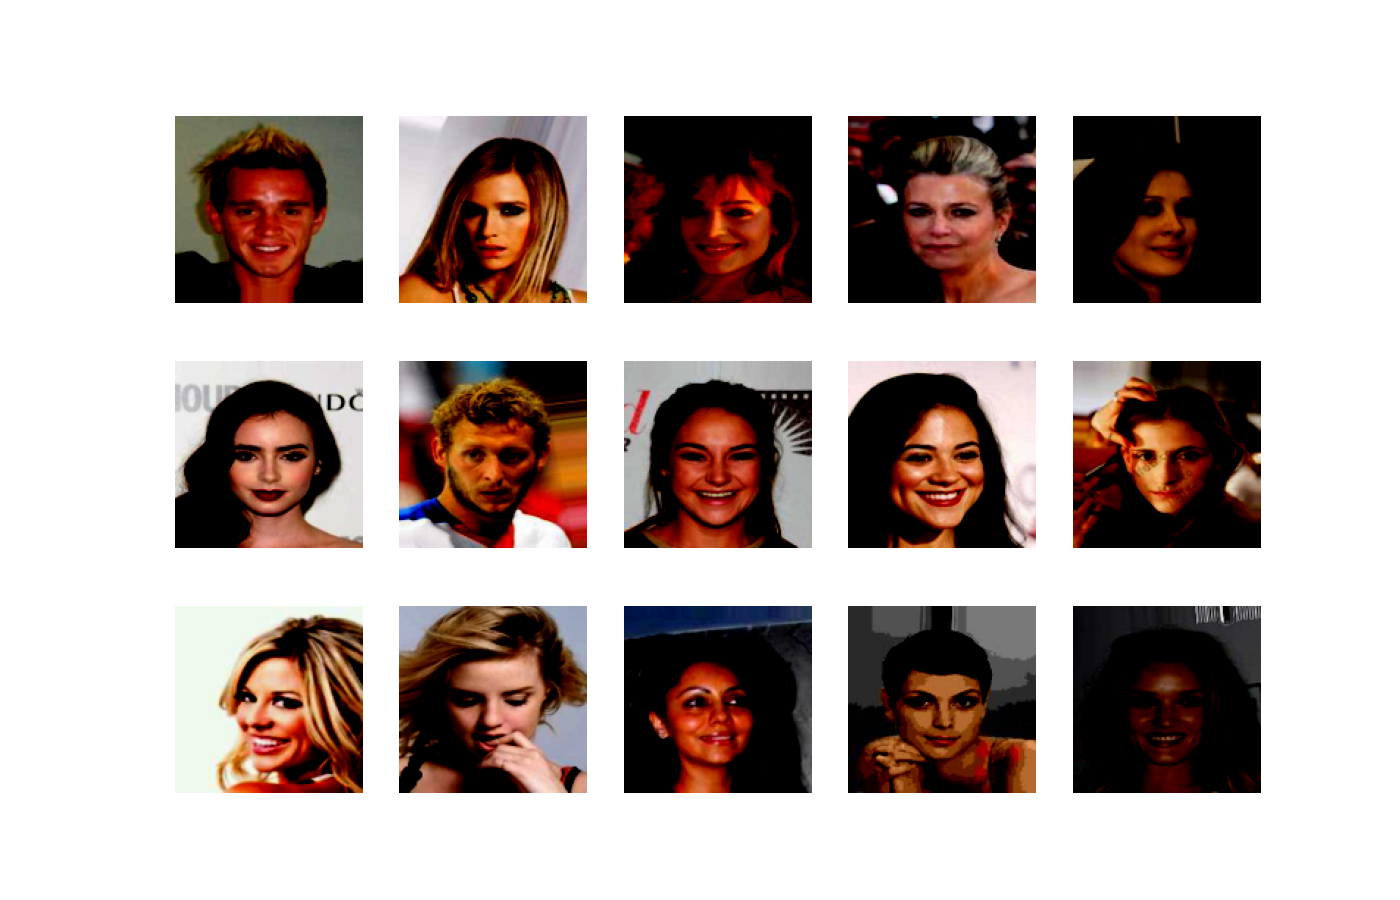
\includegraphics[width=0.8\textwidth]{./img/data_faces.png}
\caption{15 random Bilder von dem Datensatz}
\label{fig:random_faces}
\end{figure}

Diese Schritte bildeten eine grundlegende Basis für das effiziente Training meines GAN-Modells und halfen dabei, die Vielfalt und Qualität der Bilder zu demonstrieren, die für das Generieren realistischer und diverser Gesichtsbilder verwendet wurden.


Diese gründliche Vorbereitung und Überprüfung des CelebA-Datensatzes war entscheidend, um einen vollständigen Überblick über die verfügbaren Daten zu gewinnen \ref{fig:random_faces}. Nach dieser sorgfältigen Aufbereitung waren die Daten optimal vorbereitet und bereit für den Trainingsprozess meines WGAN-Modells.


\subsection{Aufbau der WGAN-Architektur}

In diesem Projekt habe ich eine Wasserstein Generative Adversarial Network (WGAN) Architektur entwickelt, die aus zwei Hauptkomponenten besteht: einem Kritiker (Critic) und einem Generator.

\subsubsection{Kritiker (Critic)}

Der Kritiker ist ein neuronales Netzwerk, das darauf trainiert wird, die vom Generator erstellten Bilder zu bewerten. Er besteht aus mehreren Schichten:

\begin{enumerate}
    \item \textbf{Konvolutionsschichten}: Diese Schichten dienen dazu, die Merkmale aus den Eingabebildern herauszufiltern. Ich habe insgesamt fünf Konvolutionsschichten verwendet, wobei jede Schicht die Bildauflösung halbiert und die Merkmalskarte vertieft.
    \item \textbf{Batch-Normalisierung}: Diese Schichten helfen, die Stabilität des Trainings zu verbessern, indem sie die Ausgaben der Konvolutionsschichten normalisieren.
    \item \textbf{Leaky ReLU-Aktivierung}: Nach jeder Konvolutionsschicht verwende ich die Leaky ReLU-Aktivierungsfunktion.
    \item \textbf{Vollständig verbundene Schicht}: Zum Schluss gibt es eine vollständig verbundene Schicht, die die Merkmale in eine einzige Zahl umwandelt, welche die Bewertung des Kritikers darstellt.
\end{enumerate}

\subsubsection{Generator}

Der Generator ist dafür verantwortlich, neue Bilder zu erzeugen. Er besteht aus:

\begin{enumerate}
    \item \textbf{Linearer Schicht}: Diese Schicht wandelt den Eingabe-Latentvektor in eine passende Form um.
    \item \textbf{Transponierte Konvolutionsschichten}: Fünf solcher Schichten vergrößern schrittweise die Merkmalskarte bis zur Zielgröße der generierten Bilder. Sie sind das Gegenteil von normalen Konvolutionsschichten.
    \item \textbf{Batch-Normalisierung und ReLU-Aktivierung}: Normalisiert die Ausgabe jeder Schicht, um das Training zu stabilisieren und zu beschleunigen. Sie hilft, Probleme wie das Verschwinden oder Explodieren von Gradienten zu vermeiden.
    \item \textbf{Tanh-Aktivierung in der Ausgabeschicht}: Die finale Schicht normalisiert die Pixelwerte des generierten Bildes.
\end{enumerate}

Diese WGAN-Architektur ermöglicht es mir, realistische Gesichtsbilder zu generieren und zu bewerten. Das Herzstück des Generators ist der Latentvektor, der zufällige Daten enthält und als Grundlage für die Bildgenerierung dient. Die Herausforderung besteht darin, den Generator so zu trainieren, dass er Bilder produziert, die realistisch genug sind, um den Kritiker zu täuschen.


\subsection{Training des WGAN-Modells}
Der Trainingsprozess meines WGAN Modells war sowohl herausfordernd als auch lehrreich. Ich begann mit dem Training des Modells auf Bildern mit einer Auflösung von 64x64 Pixeln.

Um eine effiziente und visuell aufschlussreiche Überwachung des Trainingsfortschritts zu ermöglichen, integrierte ich TensorBoard in meinen Workflow. TensorBoard diente als leistungsstarkes Tool, um eine Vielzahl von Metriken zu visualisieren, darunter der Critic-Loss und die generierten Bilder. Dies ermöglichte es mir, die Leistung des Generators zu beurteilen, ohne die Notwendigkeit, die Bilder lokal zu speichern.

Die Nutzung von TensorBoard hatte den entscheidenden Vorteil, dass ich den Trainingsverlauf in Echtzeit verfolgen konnte. Die interaktiven Diagramme und Grafiken boten tiefe Einblicke in die dynamischen Veränderungen des Modells. Insbesondere konnte ich die Entwicklung des Critic-Loss überwachen und so die Stabilität und Effizienz des Trainingsprozesses bewerten. Durch die visuelle Darstellung der vom Generator erzeugten Bilder auf TensorBoard konnte ich unmittelbare qualitative Bewertungen vornehmen, was entscheidend war, um sicherzustellen, dass das Modell realistische und vielfältige Gesichtsbilder generierte.

Die Verwendung von TensorBoard trug wesentlich zur Minimierung des Speicherbedarfs bei, da ich nicht jede generierte Bilditeration lokal speichern musste. Dies war besonders nützlich, da ich unzählige Modelle über unendliche Epochen hinweg trainierte. Mit TensorBoard konnte ich die Fortschritte meines Modells bequem überprüfen, solange ich Zugang zum Server hatte. Diese Herangehensweise war nicht nur platzsparend, sondern auch zeiteffizient, da ich schnell auf relevante Daten zugreifen und entscheiden konnte, welche Modelle am besten für weitere Trainings- oder Forschungszwecke geeignet waren.

\subsubsection{Anfängliche Herausforderungen}
Zu Beginn des Trainings erhielt ich sehr schlechte Ergebnisse, was auf einen Vorzeichenfehler in der Berechnung des Kritikerverlusts (Critic Loss) zurückzuführen war. Der Verlust des Kritikers sollte auf der Grundlage der Wasserstein-Distanz berechnet und maximiert werden, aber mein ursprünglicher Ansatz war:

\begin{verbatim}
def critic_loss(self, real_output, fake_output):
return torch.mean(real_output) - torch.mean(fake_output)
\end{verbatim}

Diese Berechnung war fehlerhaft. Mein Betreuer, Dr. Dennis Müller, wies mich darauf hin, dass die korrekte Formel eigentlich die Differenz umkehren sollte, denn der Kritiker versucht, den Unterschied zwischen den durchschnittlichen Werten, die er echten und gefälschten Daten zuweist, zu maximieren. Das bedeutet, er versucht, echten Daten hohe Werte und gefälschten Daten niedrige Werte zuzuweisen.

\begin{verbatim}
torch.mean(fake_output) - torch.mean(real_output)
\end{verbatim}

Nachdem ich diesen Fehler korrigiert hatte, begann ich, deutlich bessere Ergebnisse zu erzielen.

\subsection{Vom Heimlaptop zur Hochleistungs-Computing-Umgebung}
In den ersten drei Tagen meines Projekts, als ich das GAN-Modell auf meinem privaten Laptop trainierte, wurde mir schnell die Realität einer solchen Unternehmung bewusst. Tagsüber, während die Algorithmen arbeiteten und die Gesichter pixelweise auf meinem Bildschirm zum Leben erweckten, wurde mein Laptop zu einem ständigen Hintergrundgeräusch in unserem Zuhause. Es war ein Summen und Brummen, das nicht zu überhören war – eine stete Erinnerung an die Arbeit, die im Gange war.

Doch dieses Geräusch war nicht nur ein Beweis für die Aktivität und den Fortschritt meines Projekts, sondern wurde bald zu einem Punkt des häuslichen Diskurses. "Dein Laptop ist zu laut," hörte ich oft, gefolgt von einem halb ernsten, halb scherzhaften "Hast du es wieder vergessen auszumachen?" Diese Kommentare wurden zu einem festen Bestandteil meiner Abende, als ich mein Gerät durch die Nacht laufen ließ, in der Hoffnung, am nächsten Morgen den Fortschritt zu sehen.

Angesichts dieser Herausforderungen entschied ich mich für den Wechsel zu den Hochleistungsrechnern der Universität. Diese Umstellung ermöglichte es mir, mein Modell effizienter und schneller zu trainieren. Allerdings hatte dieser Wechsel auch seine Tücken: Ich konnte nur dann auf die Hochschulcomputer zugreifen, wenn ich physisch im Hochschulnetzwerk eingeloggt war. Dies bedeutete, dass ich an meinen freien Tagen zur Universität gehen musste, nur um den Fortschritt meines Trainings zu überprüfen.

Diese zusätzliche Anforderung machte mir die Bedeutung von Zugänglichkeit und Flexibilität in der Forschung bewusst. Während es auf der einen Seite eine Erleichterung war, die Rechenleistung zu haben, brachte es auf der anderen Seite das Bedürfnis mit sich, regelmäßig vor Ort zu sein, um den Fortschritt meines Projekts im Auge zu behalten. Diese Erfahrung lehrte mich, wie wichtig es ist, sowohl die technischen als auch die praktischen Aspekte eines Forschungsprojekts zu berücksichtigen.




\subsubsection{Auswahl des optimalen Modells}
Jedes Modell wurde in regelmäßigen Intervallen von 6000 Schritten gespeichert, was eine gründliche Analyse des Trainingsfortschritts ermöglichte. Aus einer Vielzahl von Modellen wollte ich jenes mit dem niedrigsten Critic-Loss aus, was durch die orangefarbene Linie in Abbildung \ref{fig:critic_loss} dargestellt ist. Danach habe ich einen konstanten Seed verwendet, um die Entwicklung der Modelle über die Epochen hinweg zu beurteilen. Dieser Ansatz offenbarte, dass die Unterschiede zwischen den Modellen eher marginal waren, nachdem eine anfängliche Verbesserung der Bildqualität stattgefunden hatte. Die visuelle Analyse zeigte, dass nach den ersten Epochen nur noch geringfügige Veränderungen auftraten, die kaum wahrnehmbar waren \ref{fig:epochs}.

\begin{figure}[ht]
\centering
% Erstes Bild
\begin{minipage}[t]{0.45\textwidth}
\centering
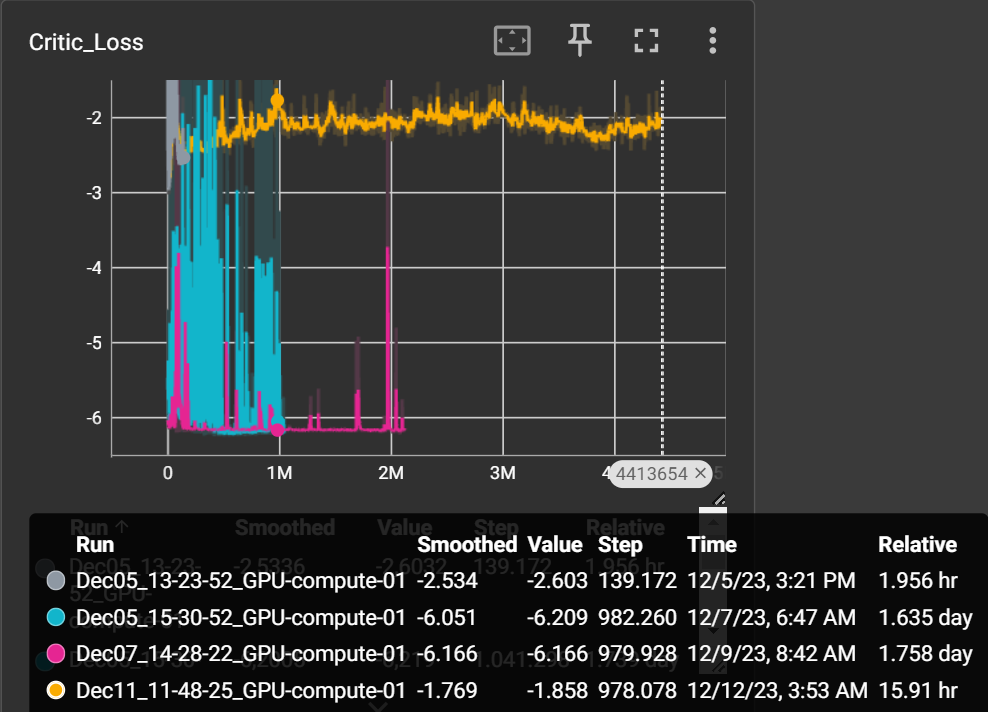
\includegraphics[height=5cm, keepaspectratio]{./img/alle_modelle.png}
\caption{Critic-Loss von den 4 verschiedenen langen Trainingverläufen}
\label{fig:critic_loss}
\end{minipage}
\hfill % Fügt einen horizontalen Zwischenraum ein
% Zweites Bild
\begin{minipage}[t]{0.45\textwidth}
\centering
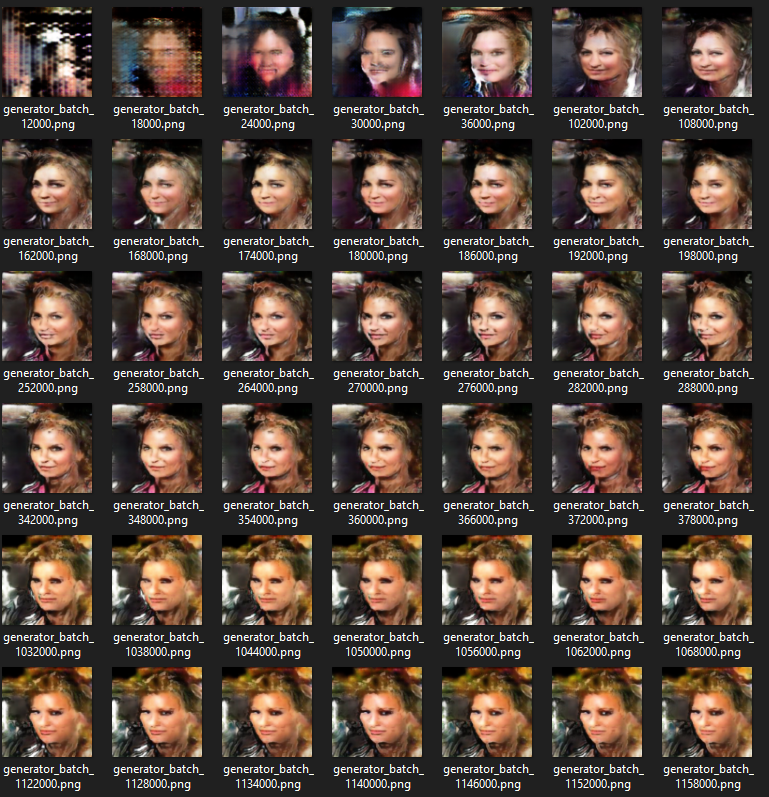
\includegraphics[height=5cm, keepaspectratio]{./img/epochs.png}
\caption{Über die Epochen hinweg generierte Bilder}
\label{fig:epochs}
\end{minipage}
\end{figure}


\subsubsection{Steigerung der Bildauflösung}
Angespornt durch diese Verbesserungen, entschied ich mich, die Auflösung der generierten Bilder schrittweise zu erhöhen, zunächst auf 128x128 und später auf 256x256 sowie 512x512 Pixel. Allerdings stieß ich dabei auf neue Herausforderungen. Anfangs funktionierte das Training mit höheren Auflösungen überhaupt nicht, was sich später als Folge einer ungeeigneten Architektur herausstellte. Nachdem ich Wochen mit erfolglosen Trainingsversuchen verbracht hatte, gelang es mir schließlich, die Architektur anzupassen und erfolgreich Bilder mit höheren Auflösungen zu trainieren.

\subsubsection{Unerwartete Ergebnisse und Entscheidungen}
Bei den Trainingsversuchen mit 256x256 und 512x512 Pixeln erhielt ich jedoch unerwartete Ergebnisse. Die generierten Bilder zeigten manchmal mehr als ein Gesicht, was auf die begrenzten Fähigkeiten von WGANs bei höheren Auflösungen hinwies. Aus diesem Grund entschloss ich mich, vorerst bei einer Auflösung von 128x128 Pixeln zu bleiben, da dies zuverlässigere und qualitativ bessere Ergebnisse lieferte.


Beim Training mit einer Auflösung von 256x256 Pixeln generierte das Modell Bilder, die zu unerwarteten Darstellungen mit mehreren Gesichtern führten, wie in Abbildung \ref{fig:multiple_faces} zu sehen ist. Dieses Phänomen unterstrich die begrenzte Fähigkeit des WGANs, bei höheren Auflösungen effektiv zu arbeiten.

Dieser Trainingsprozess des WGAN-Modells war eine intensive Lernerfahrung. Er zeigte mir die Bedeutung einer genauen Überprüfung und Anpassung der Modellarchitektur sowie die Herausforderungen, die sich beim Training von GANs mit zunehmend höheren Auflösungen ergeben.

\begin{figure}[ht]
\centering
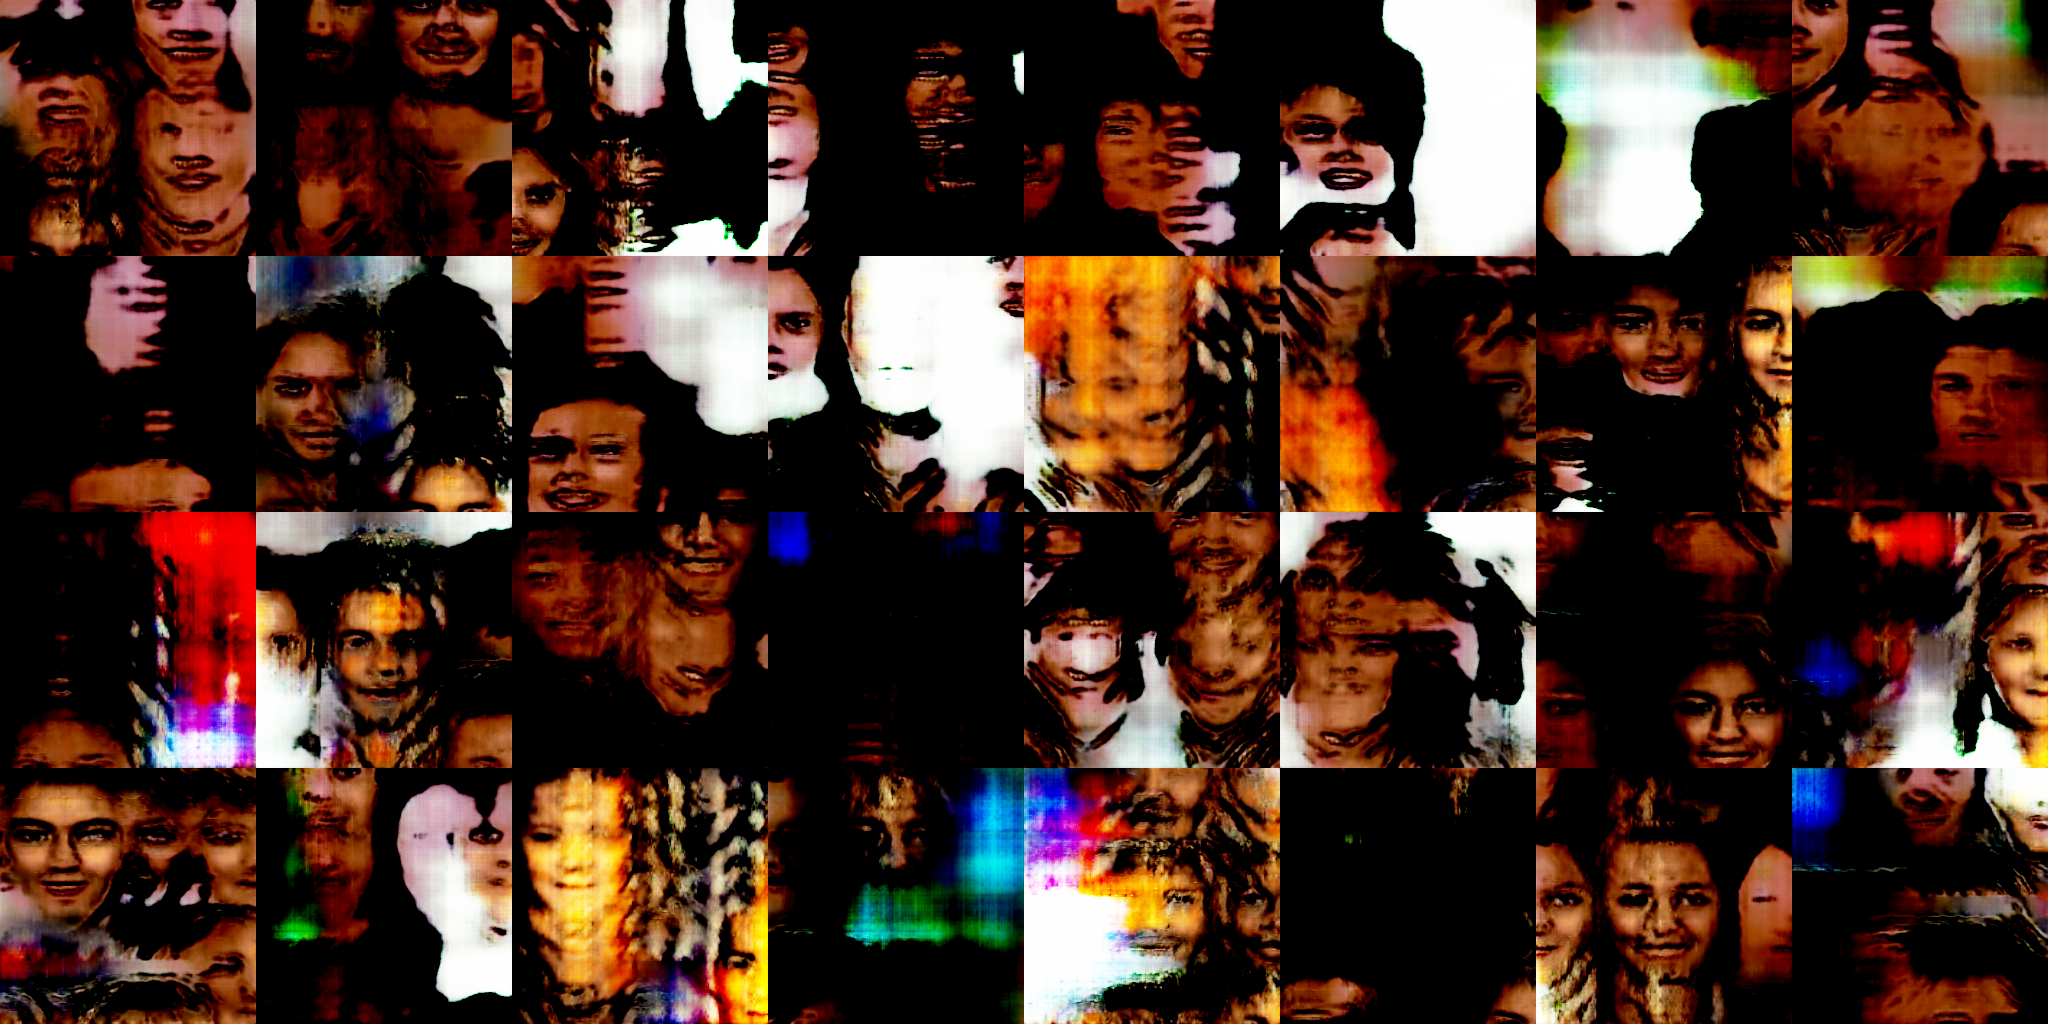
\includegraphics[width=0.8\textwidth]{./img/256x256.png}
\caption{Bei einer Auflösung von 256x256 Pixeln generierte Bilder mit multiplen Gesichtsdarstellungen.}
\label{fig:multiple_faces}
\end{figure}

Angesichts dieser Ergebnisse entschied ich mich, die Bildauflösung auf 128x128 Pixel zu beschränken, was zu einer besseren Stabilität des Modells und zuverlässigeren Ergebnissen führte. Diese Erfahrungen waren essentiell, um das Verhalten und die Grenzen des WGANs bei der Bildgenerierung zu verstehen.
Er

\section{Implementierung}
\subsection{Generierung latenter Vektoren und Interpolation}
Die Erzeugung latenter Vektoren waren zentrale Aspekte meines WGAN-Projekts. Diese Vektoren bilden die Grundlage für den Generator, um vielfältige und realistische Bilder zu erstellen.

\subsubsection{Erzeugung latenter Vektoren}
Die latenten Vektoren, die als Eingabe für den Generator dienen, erzeugte ich durch die Generierung von Zufallszahlen mittels der Funktion torch.randn in PyTorch. Diese Methode erzeugt einen Tensor mit normalverteilten Zufallszahlen. Ich wählte eine Vektorgröße von 100 (nz), da dies eine ausreichende Vielfalt für die Generierung unterschiedlicher Bilder bietet. Jeder dieser Vektoren repräsentiert einen Punkt im latenten Raum, der vom Generator verwendet wird, um ein einzigartiges Bild zu erzeugen.

\subsubsection{Interpolation zwischen Vektoren}
Die Interpolation zwischen zwei latenten Vektoren ermöglicht es, fließende Übergänge zwischen verschiedenen generierten Bildern zu erzeugen. Für diesen Zweck implementierte ich eine lineare Interpolation (Lerp). Obwohl ursprünglich geplant war, sphärische lineare Interpolation (Slerp) zu verwenden, beschränkte ich mich aufgrund zeitlicher Einschränkungen auf die einfachere lineare Interpolation. Diese Methode berechnet einen Zwischenvektor, indem sie die beiden Endvektoren linear kombiniert. Das Verhältnis der Kombination wird schrittweise verändert, um eine Sequenz von Zwischenbildern zu erzeugen, die einen glatten Übergang zwischen den vom Generator erzeugten Bildern darstellen.

Diese Technik erwies sich als effektiv, um eine visuell ansprechende Abfolge von Transformationen zwischen zwei Bildern zu schaffen, was insbesondere für die Erstellung von GIFs nützlich war. Trotz der relativen Einfachheit der linearen Interpolation bot sie dennoch die Möglichkeit, die Dynamik und das Potenzial des latenten Raumes in den generierten Bildern zu erforschen und zu demonstrieren.


\section{Ergebnisse}
In meinem Projekt habe ich sechs Gifs erstellt, die auf der Readme-Seite präsentiert. Diese Visualisierungen zeigen, was mit den entwickelten Modellen möglich ist. Um die Ergebnisse weiter zu teilen, habe ich das Anfangsmodell und vier zusätzliche Modelle auf Google OneDrive hochgeladen. Durch den Befehl \texttt{python download\_model.py} können diese Modelle heruntergeladen werden, was es jedem ermöglicht, eigene Gifs zu generieren und das Projekt vollständig zu erforschen.


\section{Next Steps}
Die nächste Schritte umfassen die Verbesserung der Übergänge im latenten Raum durch den Einsatz von slerp anstelle von lerp, was zu natürlicheren Übergängen zwischen generierten Bildern führt. Zusätzlich zielen wir darauf ab, die Qualität und Größe der Bilder durch zwei Hauptstrategien zu erhöhen: Entweder durch Weiterentwicklung des eigenen GAN-Netzwerks oder Anpassung eines vortrainierten Modells. Fortgeschrittene Techniken wie Progressive Growing of GANs, welches schrittweise die Auflösung erhöht und Self-Attention GANs, das die Beziehungen zwischen Bildteilen berücksichtigt, werden dabei eine Rolle spielen. Beide Ansätze erfordern ein sorgfältiges Feintuning und Tests, um optimale Ergebnisse zu erzielen.


\section{Zusammenfassung und Ausblick}
In meinem Projekt habe ich die Faszination und Herausforderungen von Generative Adversarial Networks (GANs) aus erster Hand erlebt, indem ich ein GAN-Netzwerk komplett von Grund auf entwickelt habe. Diese Erfahrung ermöglichte es mir, tief in die Mechanismen und Potenziale dieser Technologie einzutauchen. 

Die Auseinandersetzung mit den technischen Herausforderungen, insbesondere bei der Skalierung der Bildauflösung, hat wertvolle Einblicke in die Optimierung und Anpassung von GANs geliefert. Diese Erfahrungen bilden eine solide Grundlage für zukünftige Projekte und Forschungen in diesem Bereich.

Abschließend blicke ich mit Stolz auf das Erreichte zurück. Obwohl es in diesem rasant fortschreitenden Feld bereits fortgeschrittenere Modelle gibt, hat dieses Projekt ein solides Fundament für mein Verständnis von GANs gelegt. Die Erfahrung, ein GAN-Netzwerk von Null aufzubauen, bleibt ein unvergesslicher Meilenstein in meiner akademischen und beruflichen Entwicklung.


\section{Literaturverzeichnis}
\bibliographystyle{plain}
\bibliography{literatur}
\end{document}
